%based on https://informatik.mygymer.ch/base/?page=latex%2Fa-ma%2F
\documentclass[parskip=full]{scrreprt}
% Paket um vordefinierte Texte (z.B. "Inhaltsverzeichnis") auf Deutsch zu übersetzen
\usepackage[ngerman]{babel}

% Paket um Schriftarten festzulegen (für XeLaTeX)
\usepackage{fontspec}
%\setsansfont{OpenSans}

% serifenfreie Schriftvariante verwenden
\renewcommand{\familydefault}{\sfdefault}

% Paket um Grafiken (JPG, PNG, PDF) einzubinden
\usepackage{graphicx}

% Paket für Zeilenabstand
\usepackage{setspace}

% Paket für korrekte Anführungszeichen
\usepackage{csquotes}

% Paket für selbst definierte Kopf- und Fusszeilen
\usepackage{scrlayer-scrpage}

% Paket für Zitate und Bibliografie
%\usepackage{biblatex}

%\addbibresource{refs.bib}

% Paket zum Erzeugen von Platzhaltertext
\usepackage{lipsum}

% Used for including code snippets
\usepackage{listings}
\renewcommand{\lstlistingname}{Auflistung}
\renewcommand{\lstlistlistingname}{Auflistungsverzeichnis}
\usepackage{xcolor}
\newcommand*{\listingFont}{\ttfamily}
\newcommand*{\selectListingFont}{\listingFont\selectfont}
\lstdefinelanguage{QHS}
{
    %morekeywords={\textgreater\textgreater},
    %morecomment=[l]{//}, % l is for line comment
    morecomment=[s]{/*}{*/}, % s is for start and end delimiter
    morestring=[b]", % defines that strings are enclosed in double quotes (LiteralCode)
    %alsoletter=\textgreater
}

\definecolor{codegreen}{rgb}{0,0.6,0}
\definecolor{codegray}{rgb}{0.5,0.5,0.5}
\definecolor{codebrown}{HTML}{AB7763}
\definecolor{codeviolet}{HTML}{785175}
\definecolor{backcolour}{HTML}{CCD6E8}
\lstdefinestyle{QHSstyle}
{
    %backgroundcolor=\color{backcolour},   
    commentstyle=\color{codegreen},
    keywordstyle=\color{codeviolet},
    numberstyle=\tiny\color{codegray},
    stringstyle=\color{codebrown},
    basicstyle=\listingFont\footnotesize,
    frame=single,
    frameround=tttt,
    escapechar=\%,
    %numbers=left,
    %stepnumber=1,
}

\lstset
{
    style=QHSstyle,
    numberstyle=\listingFont
}

% Used for lines in listings
\newcommand*{\ruleEingabe}{\noindent\hrulefill { }Eingabe \noindent\hrulefill}
\newcommand*{\ruleAusgabe}{\noindent\hrulefill { }Ausgabe \noindent\hrulefill}


% Used for better float placement
\usepackage{float}

% Used for better tabulators
\usepackage{tabularx}

% Used for data figures
\usepackage{pgfplots}
% Externalize pgfplots for faster compilation
%\usepgfplotslibrary{external}
%\tikzexternalize

% Allows spliting of page into 2 parts
\usepackage{multicol}
\setlength\columnsep{20pt} % distance between columns

\usepackage{url}





% Schmale Seitenränder festlegen
\KOMAoption{DIV}{15}

% Text auf Titelseite festlegen
\subject{Maturaarbeit}
\title{Compiler Construction}
\author{Fabio Stalder\vspace{1cm}\\
Betreut durch \\
Thomas Jampen}
\publishers{
\includegraphics{resources/images/logo}\vspace{1cm}\\
Gymnasium Kirchenfeld\\
Abteilung MN}

% selbst definierte Kopf- und Fusszeile
\lohead{Maturaarbeit}
%\rohead{\theauthor}
\cofoot{\thepage}

% Zeilenabstand festlegen
\singlespacing
%\onehalfspacing
%\doublespacing

% Trennlinie für Kopfzeile
\KOMAoption{headsepline}{off}

% Trennlinie für Fusszeile
\KOMAoption{footsepline}{on}

\begin{document}

\maketitle

\tableofcontents


\iffalse
    \begin{enumerate}
        \item what is a compiler
              \begin{enumerate}
                  \item general idea
                  \item how to implement
              \end{enumerate}
        \item my different approach (QHS)
              \begin{enumerate}
                  \item define lots of macros, use lots of macros. W
                  \item write direct assembly code
                  \item only few responsibilities for Compiler
              \end{enumerate}
        \item approach for comparison
              \begin{enumerate}
                  \item 3 compilers THS, QHS and gcc
                  \item required features
                        \begin{enumerate}
                            \item output as assembly
                            \item C like syntax
                            \item variables
                            \item functions
                        \end{enumerate}
                  \item comparison
                        \begin{enumerate}
                            \item ease of use
                            \item speed of compilation
                            \item speed of assembly output
                            \item customizability, freedom and possibility for extension
                            \item error handling (required skill as a programmer)
                        \end{enumerate}
              \end{enumerate}
        \item building the compilers
              \begin{enumerate}
                  \item written in C++
                  \item THS compiler
                        \begin{enumerate}
                            \item compiler instructions in code
                            \item switch to assembly code in lexer
                            \item the Assign function problem (args for Assign function are set by calling Assign function)
                        \end{enumerate}
                  \item QHS compiler
                        \begin{enumerate}
                            \item super simple lexer
                            \item no parser
                            \item compiler instructions
                                  \begin{enumerate}
                                      \item orderStack
                                      \item typeStack
                                      \item defining identifiers
                                  \end{enumerate}
                            \item preambel defining all the stuff
                                  \begin{enumerate}
                                      \item simple shortcuts (braces, semicolons)
                                      \item more complicated stuff (classes, functions)
                                  \end{enumerate}
                        \end{enumerate}
              \end{enumerate}
    \end{enumerate}
\fi

\begin{abstract}
\lipsum[1]


\end{abstract}

\chapter{Introduction}
In der Informatik beschreibt Compiler ein Programm, das Code aus einer Programmiersprache in eine andere übersetzt. In dieser Hinsicht gleichen Compiler Übersetzern für Menschensprache.
Jedoch unterscheidet sich ein Compiler grundsätzlich von Übersetzern in der Erwartungshaltung, die an sie gestellt wird. Menschensprache ist sehr komplex und [...]

I have Idea

\chapter{Traditioneller Compiler}

Ein Compiler ist traditionell nach folgendem Schema aufgebaut.

\begin{figure}[h!]
    \centering
    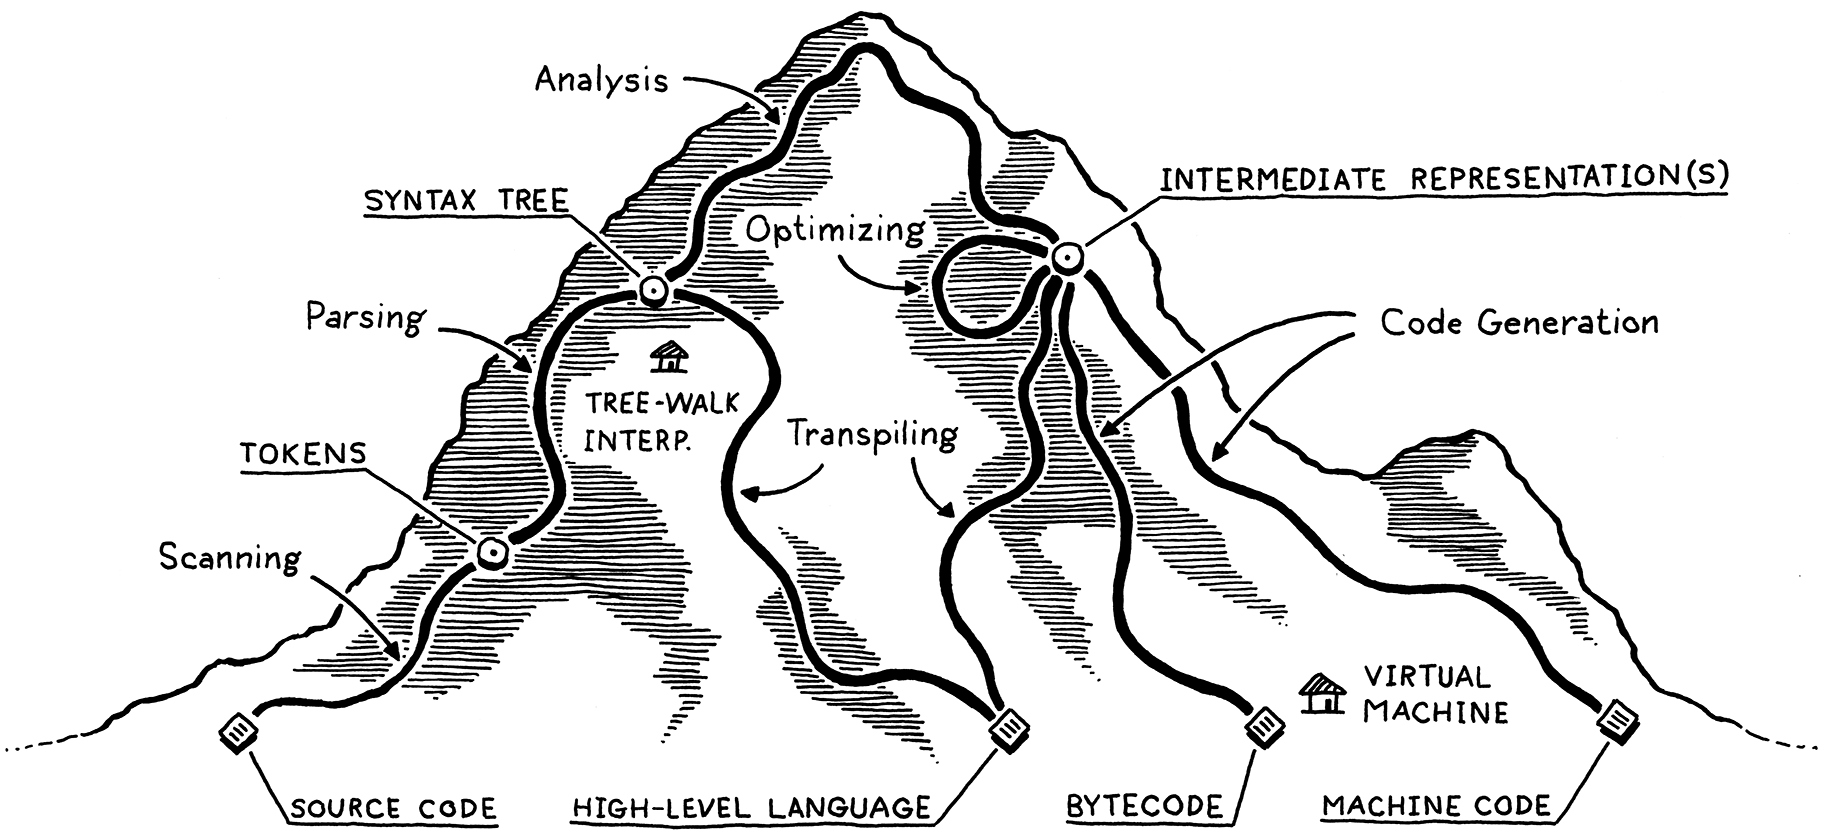
\includegraphics[scale=0.2]{resources/images/mountain.png}
    \caption[Schritte, die ein Compiler durchläuft (https://github.com/munificent/craftinginterpreters, besucht am 5.8.2024)]{Schritte, die ein Compiler durchläuft}
    \label{fig:mountain}
\end{figure}

In dieser Arbeit werde ich mich nur auf die im unteren Schema dargestellten Schritte fokussieren.

\begin{figure}[h!]
    \centering
    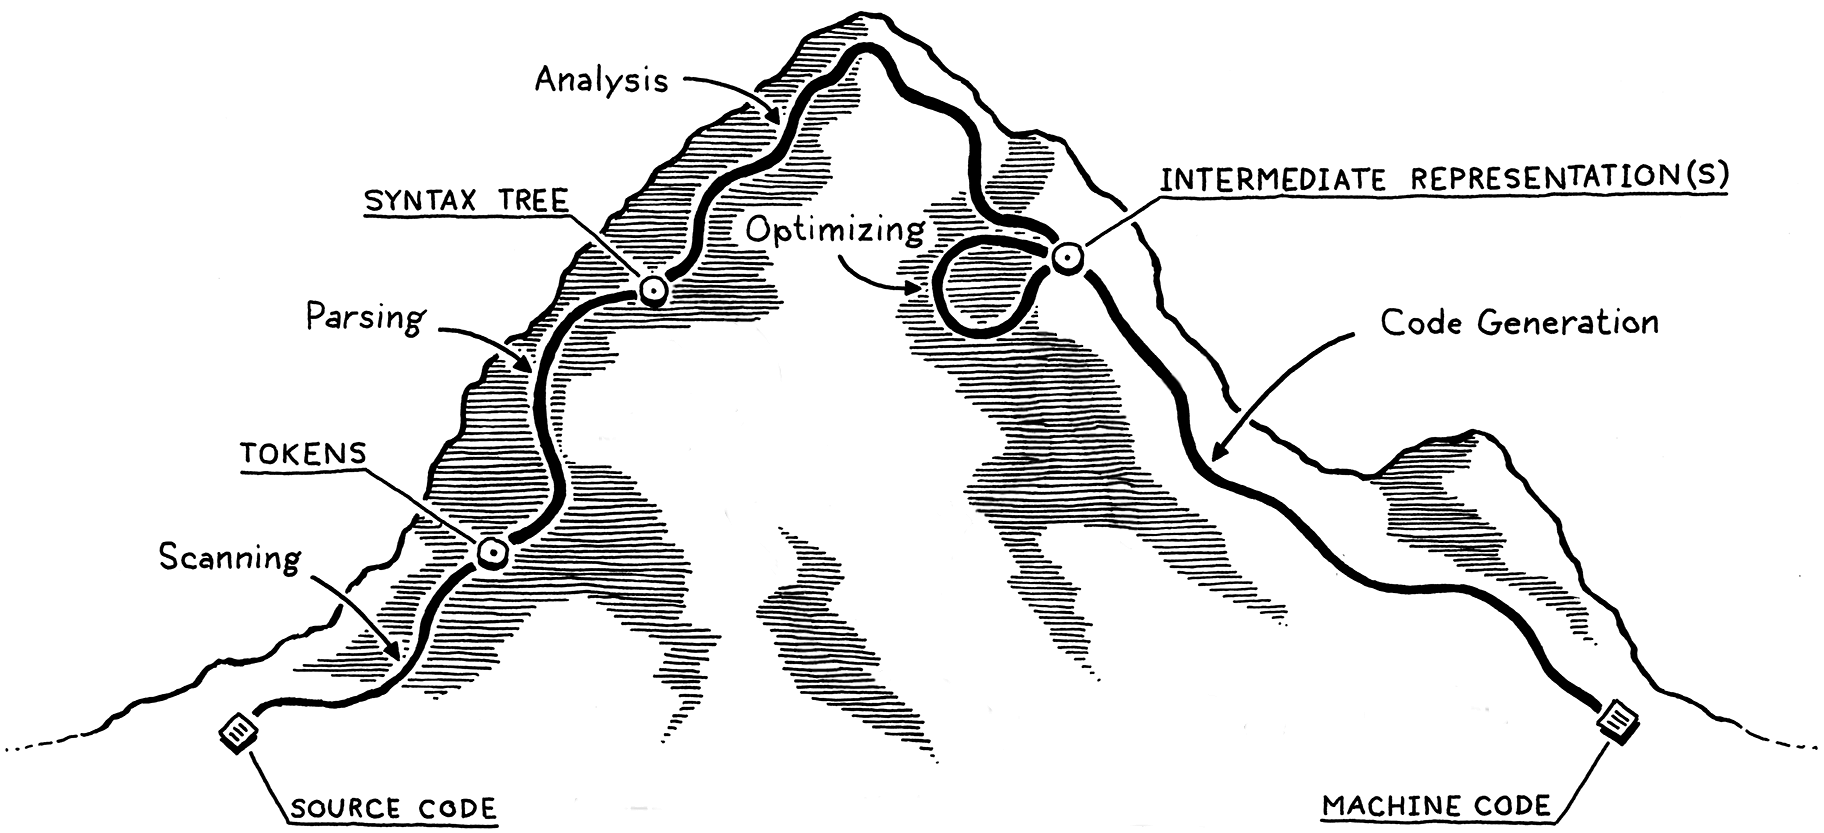
\includegraphics[scale=0.2]{resources/images/mountain-edited.png}
    \caption[Schritte, die in dieser Arbeit behandelt werden (Basierend auf Bild \ref{fig:mountain})]{Schritte, die in dieser Arbeit behandelt werden}
    \label{fig:mountain-edited}
\end{figure}

\section{Lexical Analysis}
Meist werden Programme so geschrieben, dass wir Menschen es lesen und verstehen können. Dafür verwendet man Buchstaben und Zahlen, Zeichen, wie +, *, oder Klammern, und Whitespaces, wie Leerzeichen oder Absätze.
Diese Zeichen sind jedoch für den Computer unverständlich. Der erste Schritt beim compilieren ist daher die Lexical Analysis. Dies wird von einem Teil des Compilers, dem Lexer, durchgeführt.
Die Aufgabe dieses Lexers ist es den Input File zu scannen und die gescannten Zeichen in sogenannte Tokens zu verwandeln. Diese Tokens sind Datenstrukturen, die der Compiler kennt und mit denen er weiterarbeiten kann.

Als Beispiel:

\begin{lstlisting}[language=C, label=eg:preLex, caption=C code vor Lexical Analysis]
int foo()
{
    if (bar == 0)
    {
        return 0;
    }

    return 1;
}
\end{lstlisting}

Würde hierbei zu einem Array von Token Objekten umgewandelt werden:

\begin{lstlisting}[label=eg:postLex, caption=Tokens nach Lexical Analysis]
Keyword         (keyword="int")
Identifier      (id="foo")
LParenthesis
RParenthesis
Keyword         (keyword="if")
LParenthesis
Identifier      (id="bar")
Operator        (operator=ComparisonEqual)
LiteralInt      (value=0)
[...]
\end{lstlisting}

Der Lexer legt hierbei fest welche Zeichen die Input-Programmiersprache enthalten darf und welche Bedeutung ihnen Zugesprochen wird. So ist zum Beispiel im Lexer festgelegt, dass ein + Zeichen als Addition interpretiert wird.
Genauso wie im Listing \ref{eg:postLex} 'if' als KeywordToken gesehen wird, lässt sich im Lexer auch bestimmen, dass ein Wort wie 'print' als Keyword angesehen werden soll.

\section{Syntax Analysis}
Nun versteht der Compiler was mit den Zeichen im Input File gemeint ist, jedoch fehlt noch etwas bis tatsächlich in einer andere Programmiersprache übersetzt werden kann. Und das ist Verständnis für Syntax.
Die meisten High-Level Programmiersprachen weisen Syntaxregeln auf. Diese beinhalten, wie Funktionen und Variablen definiert werden oder mit welchen Punktvorstrich-Regeln Expressions evaluiert werden.
Die bei der Lexical Analysis gefundenen Tokens werden nun ineinander verschachtelt und in einen sogenannten Abstract Syntax Tree (AST) überführt.

\begin{figure}[h!]
    \centering
    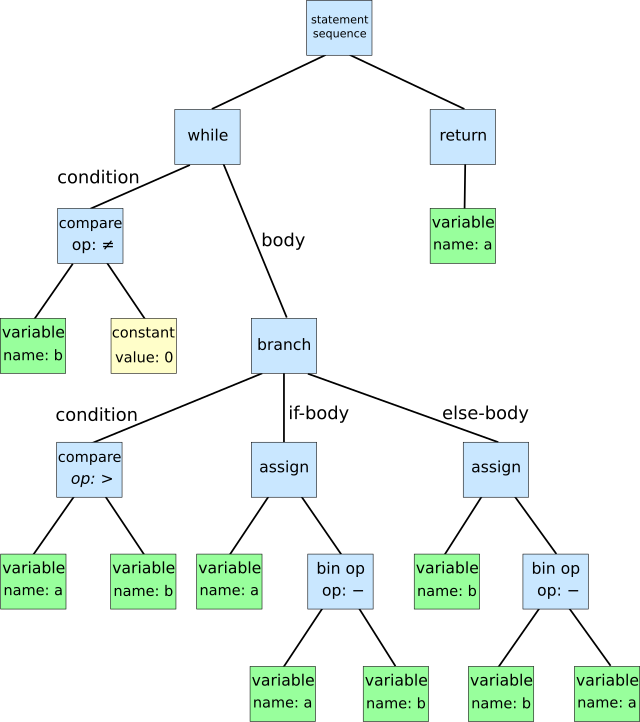
\includegraphics[scale=0.3]{resources/images/syntaxtree.svg.png}
    \caption[Abstract Syntax Tree (https://en.wikipedia.org/wiki/Abstract\_syntax\_tree, besucht am 5.8.2024)]{Abstract Syntax Tree zum Euklidischen Algorithmus}
    \label{fig:syntax-tree}
\end{figure}

Ein AST enthält somit nicht nur Informationen über die Tokens, sondern über die gesamte Struktur die sich aus den Tokens ergibt. Variabel- und Funktionsdefinitionen oder komplexe Statements wie 'if' oder 'for' sind hierbei im AST enthalten.
[...]

\section{Semantic Analysis}
Semantik ist die Wissenschaft der Bedeutung von Worten einer Menschensprache. So ähnlich ist es auch bei Programmiersprachen, jedoch geht hierbei viel weniger um Bedeutung und eher um den Datatype.
In diesem Schritt der Compilation beschäftigt sich der Compiler mit der Validität von Expressions. Unbekannte Variablen oder Funktionen werden in diesem Schritt abgefangen.
Weiter wird der Datatype einer Node an diese angebunden. Gegebenenfalls kann auch ein Implicit-Cast, also ein impliziter Wechsel des Datatypes hinzugefügt werden.
So geben zum Beispiel manche Programmiersprache bei der Division zweier Integers eine Float zurück. Wird eine Variable nicht konform ihres Datatypes verwendet, zum Beispiel die Division zweier Strings,
wird dies ebenfalls während der Semantic Analysis entdeckt und gemeldet.


\section{Code Generation}
Code Generation ist der finale und oft auch komplexeste Schritt, der ein Compiler ausführen muss. Nun da unser Input-Code nicht mehr nur als Textfile, sondern als Intermediate Representation vorliegt,
kann endlich Output-Code generiert werden. Jedoch lässt sich über diesen Schritt fast am wenigsten sagen, da er je nach Output-Sprache sehr unterschiedlich aussehen kann. 
[Code generation types]

\section{Optimization}
Code Generation ist zwar der letzte Schritt beim Compilieren, trotzdem wurde eine wichtige Aufgabe des Compilers noch nicht betrachtet. Optimization ist ein Sache die zwischen jedem der genannten Schritte geschiet
und dies häufig mehrmals. Dabei geht es darum den Output-Code so effizient wie möglich zu machen. Effizient kann hierbei jedoch viel Verschiedenes bedeuten. Der Output-Code muss so schnell wie möglich ausgeführt werden können,
Memory sparsam verwenden und am besten auch noch ein kleiner File sein. Optimization reicht vom Entfernen der Kommentare beim Scannen oder umstellen von mathematischen Operationen bis zu entfernen von ungebrauchten Variablen und Deadstores.
Es muss von CPU Registern profitiert, mit Heap-Memory umgegangen und von inline Funktionen Gebrauch gemacht werden. Compiler Optimization ist somit ein sehr vielseitiges und komplexes Problem,
dass hierbei nicht weiter thematisiert werden sollte.
\chapter{Meine Idee}
Ein Compiler ein äusserts komplexes Programm, mit vielen verschiedenen Schritten. Jedoch ist die zugrundeliegende Aufgabe gar nicht so kompliziert.
Man braucht ja nur, ein Dokument mit Text der bestimmten Regeln folgt, in Text mit anderen Regeln verwandeln. Natürlich ist dies etwas salopp ausgedrückt, trotzdem fragte ich mich,
ob es nicht möglich sei einen viel einfacheren Compiler zu schreiben. Als Grundidee 

\section{Vergleich der Compiler}
Der THS Compiler folgt dem theoretischen Aufbau eines Compilers und besteht aus Lexer, Parser und Code Generator. Als Parser wird ein Predictive Descent Parser verwendet.
Der Code Generator arbeitet auf dem Abstract Syntax Tree mithilfe eines Visitor Patterns. Die Semantic Analysis wird während der Code Generation durchgeführt. Geschrieben ist der Compiler in C++ und liefert x86 Assembly nach NASM Syntax.

Genauso wie der THScompiler ist auch der QHScompiler in C++ geschrieben und generiert x86 Assembly nach NASM Syntax.

\subsection{Anforderungen an die Compiler}
Um einen \textbf{fairen} Vergleich zu ermöglichen, müssen die Compiler folgende Anforderungen erfüllen.

\begin{table}[h]
    \begin{tabular}{l|l}
    Output als Assembly Code     & Die Output-Sprache muss Assembly Code sein                               \\
    C-like Syntax                & Die Input-Sprache muss einen C-ähnlichen Syntax aufweisen                \\
    Variablen und Funktionen     & Lokale und globale Variablen sowie Funktionen müssen unterstützt werden  \\
    Benutzerdefinierte Datatypes & Benutzerdefinierte Datatypes müssen unterstützt werden                                 
    \end{tabular}
\end{table}

Die Anforderungen machen dass Compiler gleich komplex.

\subsection{Kriterien des Vergleichs}
Die Compiler werden nach folgenden Kriterien bewertet und verglichen.

\begin{table}[h!]
    \begin{tabular}{l|l}
    Geschwindikeit des Output-Codes     & Wie schnell wird der Output-Code ausgeführt?                      \\
    Geschwindikeit der Compilation      & Wie lange dauert die Compilation von Code?                        \\
    Benutzerfreundlichkeit              & Wie einfach ist die Verwendung des Compilers?                     \\
    Möglichkeit für Erweiterung         & Wie einfach ist die Input-Sprache zu erweitern?                                 
    \end{tabular}
\end{table}
\chapter{Der QHScompiler} \label{cha:4-QHS_Compiler}
Der QHScompiler, wie in Abschnitt \ref{cha:2-Vergleich} bereits angesprochen, basiert auf einem von mir erdachten alternativen Aufbau für einen Compiler. Diesem Aufbau liegt eine einfache Idee zugrunde:
Die Macros der \textit{Macro Expansion} aus Abschnitt \ref{sec:traditional_code_generation} sollen erst während der Kompilierung innerhalb der Eingabedatei definiert werden. 
Auf dieser Grundidee werde ich zwei Dinge aufbauen. Erstens halte ich es für möglich, mit der richtigen Verwendung von Macros die gesamte syntaktische Analyse zu überspringen und keinen AST generieren zu müssen.
Zweitens sollte es rein durch die Veränderung von diesen Macros möglich sein jegliche Programmiersprache zu kompilieren. Man könnte also in einem Dokument verschiedene Programmiersprachen verwenden und
müsste dazwischen bloss die jeweiligen Macros neu definieren. Das selbige gilt ebenfalls für die Ausgabesprache.
Nur durch das Umdefinieren der Macros liesse sich die Ausgabesprache wechseln, ohne eine Änderung am Compiler vornehmen zu müssen.
Um dies zu verwirklichen, unterscheidet sich der QHScompiler stark von traditionellen Compilern.
%Um dies zu verwirklichen, folgt mein alternativer Ansatz einem Aufbau, der sich stark von einem traditionellen Compiler unterscheidet.

Die Programmiersprache, in der sich meine Macros definieren lassen, bezeichne ich als QHS. Der Compiler der QHS versteht und kompiliert, nenne ich dazu passend den QHScompiler.
QHS besteht wie die meisten anderen Programmiersprachen aus Wörtern. Im Kontext von QHS werden diese Wörter \textit{Orders} genannt.
Orders können drei verschiedenen Typen aufweisen: \textit{Identifiers}, \textit{Instructions} und \textit{LiteralCode}.
%Bei \textit{Identifiers} handelt es sich um die bereits erwähnten Macros, \textit{Instructions} sind einfache vorprogrammierte Anweisungen an den QHScompiler und \textit{LiteralCode} ist Text, der unverändert in die Ausgabedatei geschrieben wird.
Wie diese drei \textit{Ordertypen} genau funktionieren, wird in Abschnitt \ref{sec:qhs-execute} ausführlicher erklärt.

Der Kompilierung durch den QHScompiler steht ein einfacher Zyklus (\textit{QHS-Zyklus}) zugrunde, dessen Inspiration der Von-Neumann Zyklus ist.

\begin{figure}[h!]
    \centering
    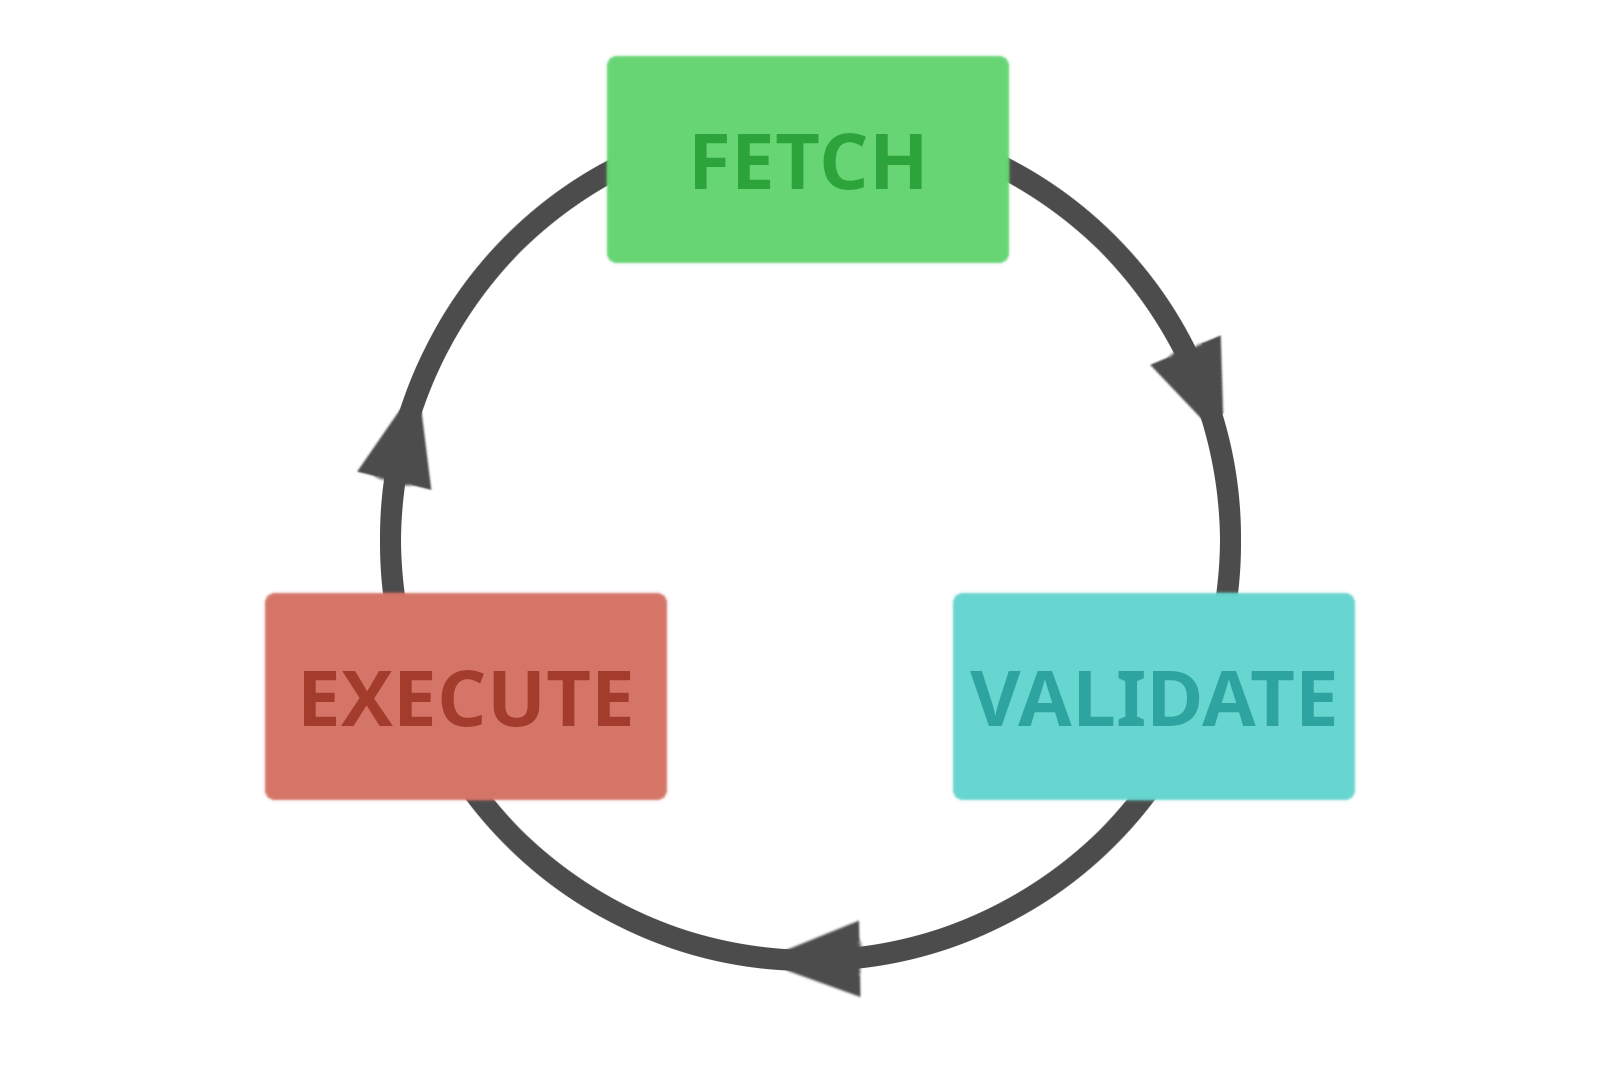
\includegraphics[scale=0.6]{resources/images/qhs-cycle.png}
    \caption{Zyklus der QHS Kompilierung}
    \label{fig:qhs-cycle}
\end{figure}

\section{Die \textit{Fetch-Phase}} \label{sec:qhs-fetch}
Die Aufgabe der \textit{Fetch-Phase} ist es die nächste \textit{Order}, die verarbeitet werden soll, zu finden. In dieser Hinsicht gleicht die \textit{Fetch-Phase} der lexikalischen Analyse eines traditionellen Compilers.
Der QHS-Zyklus beginnt bei der \textit{Fetch-Phase}, dabei wird die erste \textit{Order} aus der Eingabedatei extrahiert. In jeder weiteren \textit{Fetch-Phase} wird die nächste \textit{Order} aus der Eingabedatei geholt.
Die \textit{Fetch-Phase} ist auch dafür zuständig die nächste \textit{Order} einem der drei Typen (\textit{Identifier}, \textit{Instruction} oder \textit{LiteralCode}) zuzuordnen.
Diese \textit{Ordertypen} sind mit folgenden Regular-Expressions definiert. Leerzeichen dienen als Trennung zwischen \textit{Orders} und werden ignoriert.

\begin{table}[h]
    \fontsize{13}{17}\selectfont
    \centering
    \caption{RegEx Definitionen der \textit{Ordertypen}}
    \vspace{3mm} % Adjust the height of the space between caption and tabular
    
    \begin{tabular}{l>{\listingFont\selectfont}l}
    \multicolumn{1}{l|}{identifier}        & {[}\textasciicircum \textbackslash{}s{]}+                         \\ \hline
    \multicolumn{1}{l|}{instruction}       & \#{[}\textasciicircum \textbackslash{}s{]}+                      \\ \hline
    \multicolumn{1}{l|}{literalCode}       & ".*"                                                              \\
    %                                       &                                                                   \\
    %\textless{}identiferChar\textgreater{} & = {[}\textasciicircum{}\# "\textless{}whitespace\textgreater{}{]} \\
    %\textless{}whitespace\textgreater{}    & = SPACE | NEWLINE | TAB
    
    \end{tabular}
\end{table}

Im Vergleich zu traditionellen Compilern fällt auf, dass beim QHScompiler kaum zwischen Zeichen differenziert wird. Während die lexikalische Analyse traditionell zwischen vielen verschiedenen \textit{Tokens} unterscheidet,
sind für den QHScompiler alle Zeichen (mit Ausnahme von {\listingFont\selectfont \#} und {\listingFont\selectfont "{}}) gleichbedeutend.

Normalerweise erhält die \textit{Fetch-Phase} die nächste \textit{Order} aus der Eingabedatei. 
Es ist jedoch möglich \textit{Orders} der Eingabedatei voranzustellen. Diese \textit{Orders} werden in der \textit{Fetch-Phase} zuerst gefunden. Dies geschieht mithilfe des \textit{FetchStacks}, auf den \textit{Orders} gelegt werden können.
In der nächsten \textit{Fetch-Phase} wird immer die oberste \textit{Order} des \textit{FetchStacks} geholt und daraufhin vom \textit{FetchStack} entfernt.
Die Eingabedatei befindet sich auf dem untersten Platz des \textit{FetchStacks} und wird somit nur verwendet, wenn der Stack ansonsten komplett leer ist.
%Eine \textit{Order} kann während jedem der drei Schritte des QHS-Zyklus auf den \textit{FetchStack} gelegt werden.

%FETCHSTACK FIGURE

%Während der Laufzeit des QHScompilers könnte der \textit{FetchStack} folgendermassen aussehen:
%
%\begin{figure}[h!]
%    \centering
%    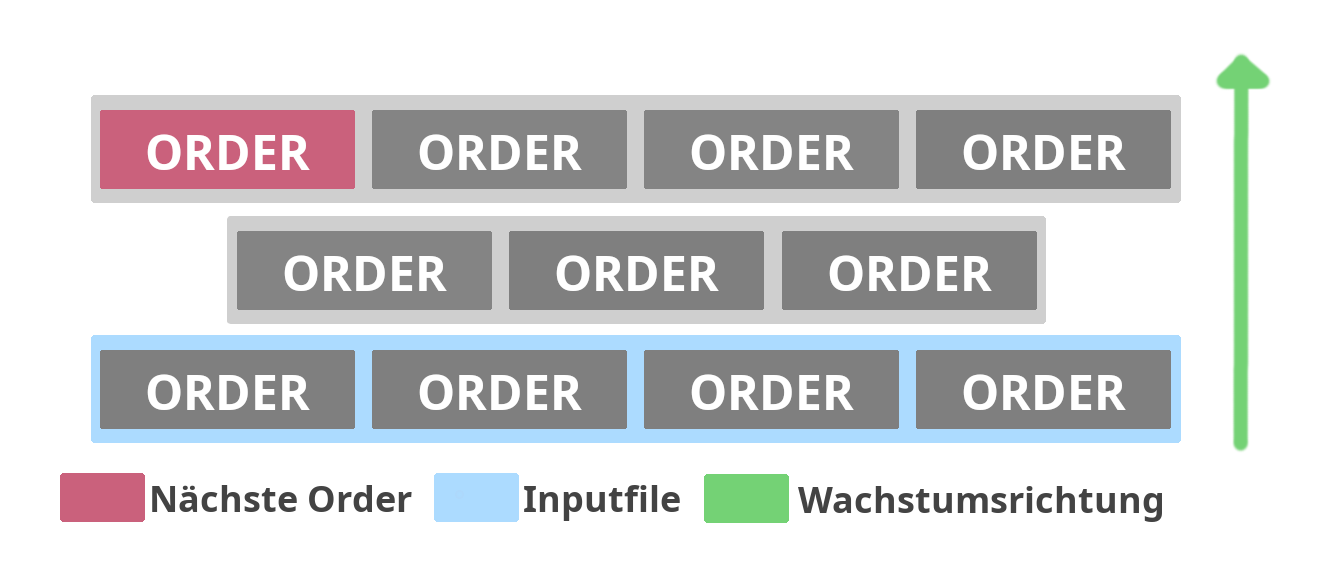
\includegraphics[scale=1.1]{resources/images/fetch-stack.png}
%    \caption{Struktur des \textit{FetchStacks} UPDATE}
%    \label{fig:fetchstack}
%\end{figure}
%
Die Hauptanwendung des \textit{FetchStacks} wird im Abschnitt \ref{sec:qhs-execute} erklärt.
Die Kompilierung ist beendet, sobald keine \textit{Order} mehr auf dem \textit{FetchStack} vorhanden ist.

\section{Die \textit{Validate-Phase}} \label{sec:qhs-Validate}
Nachdem die nächste \textit{Order} in der  \textit{Fetch-Phase} gefunden wurde, wird diese \textit{Order} an die \textit{Validate-Phase} weitergegeben. Während der \textit{Validate-Phase} kommt die \textit{OrderQueue} ins Spiel.
Dabei handelt es sich, wie der Name schon sagt, um eine Queue von \textit{Orders}.
Die Aufgabe der \textit{OrderQueue} ist das Speichern und spätere Zurückholen von \textit{Orders}.
Die \textit{OrderQueue} kann mit \textit{Instructions}, die im Abschnitt \ref{sec:qhs-execute} weiter ausgeführt werden, aktiviert und deaktiviert werden.
Wenn eine \textit{Order} in die \textit{Validate-Phase} gelangt und die \textit{OrderQueue} aktiviert ist, wird diese \textit{Order} der \textit{OrderQueue} hinzugefügt.
Die \textit{Execute-Phase} wird danach übersprungen und der QHS-Zyklus beginnt von neuem bei Fetch.
Die \textit{Order} wurde (ohne die \textit{Execute-Phase} erreicht zu haben) auf der \textit{OrderQueue} gespeichert.
Später ist es mit \textit{Instructions} möglich diese \textit{Order} von der \textit{OrderQueue} zu entfernen und auszuführen.

Bestimmte \textit{Orders} können jedoch \textit{orderQueue-proof}, also immun gegen die \textit{OrderQueue}, gemacht werden.
\textit{Orders}, die \textit{orderQueue-proof} sind, werden an die \textit{Execute-Phase} weitergegeben, auch wenn die \textit{OrderQueue} aktiv ist.
Dieses Prinzip ist zum Beispiel besonders bei der \textit{Instruction}, welche die \textit{OrderQueue} wieder deaktiviert, wichtig.
Da diese \textit{Instruction} ansonsten nicht zur \textit{Execute-Phase} gelänge und somit die \textit{OrderQueue} nie deaktiviert würde.
Zu beachten ist, dass \textit{LiteralCode} nicht \textit{orderQueue-proof} sein kann.

%MAYBE OrderQueue FIGURE

Ist die \textit{OrderQueue} deaktiviert oder die \textit{Order} \textit{orderQueue-proof}, gelangt diese \textit{Order} zur \textit{Execute-Phase}.

\section{Die \textit{Execute-Phase}} \label{sec:qhs-execute}
Während der \textit{Execute-Phase} wird der tatsächliche Assembly-Code generiert. Je nach Typ der \textit{Order} (\textit{Identifier}, \textit{Instruction} oder \textit{LiteralCode}) läuft die \textit{Execute-Phase} sehr unterschiedlich ab.
In den folgenden Abschnitten wird der Ablauf der \textit{Execute-Phase} je nach \textit{Ordertyp} erklärt.

\subsection{\textit{Identifier} in der \textit{Execute-Phase}}
\textit{Identifier} stehen für die am Anfang von Abschnitt \ref{cha:4-QHS_Compiler} erwähnten Macros.
Die Macros sind für den QHScompiler eine Liste an \textit{Orders}.
\textit{Identifier} lassen sich zu einer Liste an \textit{Orders} definieren.
Wenn nun ein \textit{Identifier} in die \textit{Execute-Phase} gelangt, werden die dazugehörigen \textit{Orders} auf den \textit{FetchStack} aus Abschnitt \ref{sec:qhs-fetch} gelegt.
Bei den nächsten \textit{Fetch-Phasen} werden nun zuerst die zum \textit{Identifier} gehörenden \textit{Orders} nacheinander abgebaut. Einfach ausgedrückt wird der \textit{Identifier} also durch seine \textit{Orders} ersetzt.
Als Beispiel seien folgende \textit{Identifier} definiert:

\begin{table}[H]
    \centering
    \caption{Definition von \textit{Identifiern} als Beispiel}
    \vspace{3mm} % Adjust the height of the space between caption and tabular    
    
    \begin{tabular}{l|l}
    \textbf{Identifier} & \textbf{Definition}   \\ \hline
    \listingFont\selectfont id1 & \listingFont\selectfont "lit1"                                \\ \hline
    \listingFont\selectfont id2 & \listingFont\selectfont \#inst2.1 "lit2" { }\#inst2.2         \\ \hline
    \listingFont\selectfont id3 & \listingFont\selectfont id2 "lit3"     
    \end{tabular}
\end{table}

Mit diesen \textit{Identifiern}, wird nun folgender Code kompiliert:

\begin{lstlisting}[language=QHS, caption=QHS-Code zur Veranschaulichung von \textit{Identifiern}]
%\ruleEingabe%
"lit0.1"
id1
"lit0.2" id2
id3
%\ruleAusgabe%
"lit0.1"
"lit1"
"lit0.2" #inst2.1 "lit2" #inst2.2
#inst2.1 "lit2" #inst2.2 "lit3"
\end{lstlisting}

Die \textit{Identifier} aus der Eingabe wurden mit ihren Definitionen ersetzt. Wie der \textit{Identifier} {\listingFont\selectfont id3} zeigt, ist es möglich \textit{Identifier} ineinander zu verschachteln.

Die Definitionen der \textit{Identifier} sind in einem sogenannten \textit{Environment} definiert.
Bei einem \textit{Environment} handelt es sich um eine einfache Map, die einen \textit{Identifier} mit einer Liste an \textit{Orders} verknüpft.
\textit{Environments} sind in einer verketteten Liste gespeichert. Neue \textit{Environments} können dieser Liste hinzugefügt und aus der Liste entfernt werden.
Das letzte \textit{Environment} der Liste ist das älteste und das erste \textit{Environment} das neuste.
Ein neuer \textit{Identifier} wird immer zum ersten \textit{Environment} der Liste hinzugefügt. Definitionen des gleichen \textit{Identifiers} in älteren \textit{Environments} werden nicht überschrieben oder gelöscht.
Bei der Abfrage nach einem \textit{Identifier} wird immer die neuste vorhandene Definition zurückgegeben.
In Abschnitt \ref{sec:howto-identifiers} werden \textit{Environments} anhand eines Beispiels erneut aufgegriffen.

\subsection{\textit{Instruction} in der \textit{Execute-Phase}}
%\textit{Instructions} sind die komplexesten \textit{Orders} für die \textit{Execute-Phase}. 
Wenn eine \textit{Instruction} in die \textit{Execute-Phase} gelangt, wird die dazu definierte Funktion im QHScompiler ausgeführt.
Diese Funktionen können \textit{Identifier} definieren, die \textit{OrderQueue} aktivieren, Zahlen addieren und vieles mehr.
\textit{Instructions} sind somit der Weg wie während der Kompilierung auf den QHScompiler Einfluss genommen werden kann.
In der Tabelle \ref{tab:important_instructions} sind ein paar der wichtigsten \textit{Instructions} aufgelistet:

\begin{table}[H]
    \centering
    \caption{Wichtige Instructions des QHScompilers}
    \label{tab:important_instructions}
    \vspace{3mm} % Adjust the height of the space between caption and tabular
    
    \begin{tabularx}{\textwidth}{l|X}
    \textbf{Instruction}                             & \textbf{Beschreibung} \\ \hline
    {\listingFont\selectfont \#enterOrderQueue}      & Aktiviert die \textit{OrderQueue}. Diese \textit{Instruction} ist \textit{orderQueue-proof}. \\ \hline
    {\listingFont\selectfont \#exitOrderQueue}       & Deaktiviert die \textit{OrderQueue}. Diese \textit{Instruction} ist \textit{orderQueue-proof}. \\ \hline
    {\listingFont\selectfont \#assign}               & Die erste \textit{Order} der \textit{OrderQueue} muss ein \textit{Identifier} sein.
                                                       Der Rest der \textit{Orders} auf der \textit{OrderQueue} wird als Definition für diesen \textit{Identifier} festgelegt. \\ \hline
    {\listingFont\selectfont \#assignToOne}          & Wie {\listingFont\selectfont \#assign}, jedoch wird nach dem \textit{Identifier} nur eine weitere \textit{Order} von der \textit{OrderQueue} genommen und 
                                                       als Definition für den \textit{Identifier} verwendet. \\ \hline
    {\listingFont\selectfont \#force}                & Die nächste \textit{Order} wird nach der \textit{Fetch-Phase} sofort an die \textit{Execute-Phase} weitergegeben.
                                                       Überspringt die \textit{Validate-Phase} und somit die \textit{OrderQueue}. Diese \textit{Instruction} ist \textit{orderQueue-proof}. \\ \hline
    %{\listingFont\selectfont \#lightForce}           & Ähnlich wird {\listingFont\selectfont \#force}, jedoch wird diese nur ausgeführt, wenn \textbf{explain this cuz they don't know OrderQueue depth} \\ \hline
    {\listingFont\selectfont \#orderEnqueue}         & Die nächste \textit{Order} wird sofort dem Ende der \textit{OrderQueue} hinzugefügt, auch wenn diese \textit{Order} \textit{orderQueue-proof} wäre.
                                                       Die \textit{Execute-Phase} wird übersprungen. \\ \hline
    {\listingFont\selectfont \#orderFrontEnqueue}    & Ähnlich wie {\listingFont\selectfont \#orderEnqueue}. Die \textit{Order} wird jedoch an den ersten Platz der \textit{OrderQueue} gesetzt. \\ \hline
    {\listingFont\selectfont \#deepFetch}            & Die nächste \textit{Order} der Eingabedatei wird oben auf den \textit{FetchStack} gesetzt. Ermöglicht den Zugriff auf die Eingabedatei innerhalb eines \textit{Identifiers}. \\ \hline
    {\listingFont\selectfont \#queueFetch}           & Die erste \textit{Order} der \textit{OrderQueue} wird oben auf den \textit{FetchStack} gesetzt. \\ \hline 
    {\listingFont\selectfont \#pushEnv}              & Ein neues \textit{Environment} wird der \textit{Environment-Liste} hinzugefügt. \\ \hline
    {\listingFont\selectfont \#popEnv}               & Das neuste \textit{Environment} der \textit{Environment-Liste} wird gelöscht. \\ \hline
    {\listingFont\selectfont \#addToIdentifier}      & Die erste \textit{Order} der \textit{OrderQueue} muss ein \textit{Identifier} sein und die zweite \textit{LiteralCode}. Die Definition des \textit{Identifiers} muss eine Zahl sein.
                                                       Der \textit{LiteralCode} wird zu dieser Zahl addiert und im \textit{Identifier} gespeichert.       
    \end{tabularx}
\end{table}

Der QHScompiler umfasst 33 \textit{Instructions}, wobei 5 dieser ausschliesslich fürs Debuggen des Compilers dienen.

\subsection{\textit{LiteralCode} in der \textit{Execute-Phase}}
\textit{LiteralCode} ist der Weg wie der QHScompiler Assembly-Code generiert. Dieser ist sehr einfach.
Wenn \textit{LiteralCode} in die \textit{Execute-Phase} gelangt, wird alles, das zwischen den Satzzeichen steht, in die Ausgabedatei geschrieben.
Dies ist die einzige Möglichkeit des QHScompiler Assembly-Code zu generieren. Einzig die \textit{LiteralCode-Orders} bestimmen, was in die Ausgabedatei gelangt, und somit welcher Sprache diese Ausgabedatei folgt. 
Durch das Anpassen der \textit{LiteralCode-Orders} ist es also möglich die Ausgabesprache des QHScompilers zu ändern.


\section{Definition der Macros} \label{sec:qhs-macro_definitions}
Somit ist der QHScompiler komplett. Grundsätzlich lässt sich mit \textit{LiteralCode} bereits jedes Programm schreiben und mit dem QHScompiler kompilieren. 
Jedoch habe ich in Abschnitt \ref{cha:2-Vergleich} festgelegt, dass die Eingabesprache einen C ähnlichen Syntax aufweisen und die Ausgabesprache Assembly sein muss.
Um dies zu ermöglichen, muss man, wie zu Beginn von Abschnitt \ref{cha:4-QHS_Compiler} erwähnt, bestimmte Macros also \textit{Identifier} definieren.
In diesem Abschnitt werde ich zeigen, wie sich diese \textit{Identifier} auch für syntaktisch komplexe Programmiersprachen definieren lassen.
Zur Veranschaulichung dienen Variablen und Funktionsdefinitionen.


\iffalse
Der QHScompiler ist zwar komplett, die dazugehörige Programmiersprache QHS jedoch noch lange nicht.
Grundsätzlich ist es möglich mit \textit{LiteralCode} jedes Programm zu schreiben und zu kompilieren, jedoch handelt es sich dann nur um Assembly-Code.
Doch der Aufbau des QHScompilers ermöglicht es mit \textit{Identifiern} eine komplexere Programmiersprache zu definieren. Ein fester Bestandteil ein jedes Programms, das mit dem QHScompiler kompiliert werden soll, ist ein Stück Code,
das die jeweilige Programmiersprache definiert. Dieser Code wird im Kontext des QHScompilers \textit{Preamble} genannt. Theoretisch ist es möglich durch das Anpassen dieses Preambles, 
viele unterschiedliche Programmiersprachen mit dem QHScompiler zu kompilieren. In diesem Abschnitt wird behandelt wie sich die Sprache QHS, welche die Kriterien aus Abschnitt \ref{sec:Vergleichs_Kriterien} erfüllt,
für den QHScompiler definieren lässt.
\fi

\subsection{Die QHS Notation} \label{sec:qhs-notation}
In diesem Abschnitt wird viel QHS-Code als Beispiel verwendet.
Um die Leserlichkeit von QHS zu verbessern, werden zuerst paar \textit{Identifier} anstelle der umständlichen \textit{Instructions} definiert.
Diese \textit{Identifier} sind in der folgenden Tabelle \ref{tab:shortcuts} aufgeführt.

{
\begin{table}[H]
    \centering
    \caption{\textit{Identifier} als Abkürzung von \textit{Instructions}}
    \vspace{3mm} % Adjust the height of the space between caption and tabular
    \label{tab:shortcuts}
    
    \begin{tabular}{l|l}
    \textbf{Identifier}                                     & \textbf{Definition}            \\ \hline
    {\listingFont\selectfont [}                             & {\listingFont\selectfont \#enterOrderQueue}              \\ \hline
    {\listingFont\selectfont ]}                             & {\listingFont\selectfont \#exitOrderQueue}               \\ \hline
    {\listingFont\selectfont \textgreater{}\textgreater{}}  & {\listingFont\selectfont \#assign}                       \\ \hline
    {\listingFont\selectfont -\textgreater{}}               & {\listingFont\selectfont \#assignToOne}                  \\ \hline
    {\listingFont\selectfont !}                             & {\listingFont\selectfont \#force}                        \\ \hline
    %{\listingFont\selectfont ?!}                            & {\listingFont\selectfont \#lightForce}                   \\ \hline
    {\listingFont\selectfont \textbackslash{}n}             & Eine neue Zeile in der Ausgabedatei
    \end{tabular}
\end{table}
}

Weiter wird innerhalb von Kommentaren Pseudo-Code verwendet, um den QHS-Code verständlicher zu erklären.
Kommentare können mehrere Zeilen umfassen und beginnen immer mit {\listingFont\selectfont /*} und enden mit {\listingFont\selectfont*/}.
Der Kommentar {\listingFont\selectfont /* X = "test" { }\#pushEnv */} würde bedeuten,
dass der \textit{Identifier} {\listingFont\selectfont X} zu den \textit{Orders} {\listingFont\selectfont "test"{}} (\textit{LiteralCode}) und {\listingFont\selectfont \#pushEnv} (\textit{Instruction}) definiert wurde. 

Auch wird bei längeren \textit{Identifier}-Definitionen wird zuerst der zu definierende \textit{Identifier} getrennt von den restlichen \textit{Orders} der \textit{OrderQueue} hinzugefügt.
Diese Separation dient der besseren Leserlichkeit und hat keinen Einfluss auf die Kompilierung des Codes.

\subsection{Beispiele zu \textit{Identifier}-Definitionen} \label{sec:howto-identifiers}
Wie die Definition von \textit{Identifiern} ablaufen kann, wird hier an einigen Beispielen erklärt.

\begin{minipage}{\linewidth}
\begin{multicols}{2}
\begin{lstlisting}[language=QHS, label=eg:howto_id1-3, caption=Beispiel zu gewöhnlichen \textit{Identifier}-Definitionen, numbers=left, stepnumber=1]
%\ruleEingabe%
[ id1 "lit1" ] ->
[ id2 "lit2.1" "lit2.2" id1 ] >>
[ id3 "lit3.1" ] [ "lit3.2" ] >>

id1 \n
id2 \n
id3

%\ruleAusgabe%

lit1
lit2.1 lit2.2 lit1
lit3.1 lit3.2
\end{lstlisting}
\columnbreak
\iffalse
    In Linie 1 wird zuerst die \textit{OrderQueue} geöffnet und die Orders {\selectListingFont id1} und {\selectListingFont "lit1"{}} hinzugefügt.
    Schliessen sieht die \textit{OrderQueue} wie folgt aus:
    \centerline{\selectListingFont id1 "lit1"{}}
    Mit {\selectListingFont ->} wird die erste \textit{Order} der \textit{OrderQueue} ({\selectListingFont id1}) zu der zweiten \textit{Order} ({\selectListingFont "lit1"{}}) definiert.
    \break
    In Linie 2 kommt {\selectListingFont id2}, {\selectListingFont "lit2"{}}, {\selectListingFont \#inst2} und {\selectListingFont id1} auf die \textit{OrderQueue}. Diese sieht daraufhin wie folgt aus:
    \centerline{\selectListingFont id2 "lit2"{} \#inst2 id1}
    Der Identifier {\selectListingFont >>} definiert die erste \textit{Order} der \textit{OrderQueue} ({\selectListingFont id2}) zu allen restlichen \textit{Order} auf der \textit{OrderQueue}.
    Die Definition von {\selectListingFont id2} ist daraufhin:
    \centerline{\selectListingFont id2 = "lit2"{} \#inst2 id1}
\fi
Die Linien 2 und 3 definieren die folgenden beiden \textit{Identifier}: \break
\centerline{\selectListingFont id1 = "lit1"{}}
\centerline{\selectListingFont id2 = "lit2.1"{} "lit2.2"{} id1}
In Linie 4 wird die \textit{OrderQueue} zwischendurch deaktiviert und wieder aktiviert.
Dies hat keinen Einfluss auf die Kompilierung und wird daher, wie in Abschnitt \ref{sec:qhs-notation} erwähnt, für die Verbesserung der Leserlichkeit von langen \textit{Identifier}-Definitionen verwendet.
Die \textit{OrderQueue} sieht vor dem {\selectListingFont >>} wie folgt aus, wobei das linkste Element das erste darstellt:  \break
\centerline{\selectListingFont id3 "lit3.1"{} "lit3.2"{}}
Wie gewohnt wird {\selectListingFont id3} mit {\selectListingFont >>} definiert: \break
\centerline{\selectListingFont id3 = "lit3.1"{} "lit3.2"{}}
\end{multicols}
\end{minipage}
\vspace{\baselineskip}

\begin{minipage}{\linewidth}
\begin{multicols}{2}
\begin{lstlisting}[language=QHS, caption=Beispiel zu {\selectListingFont \#assignToOne}, numbers=left, stepnumber=1]
%\ruleEingabe%
[ id4 "lit4" ] >>
[ id5 "lit5" id6 ] ->
[ "lit6" ] >>

id4 \n
id5 \n
id6



%\ruleAusgabe%

lit4
lit5
lit6
\end{lstlisting}
\columnbreak
Die Definition von {\selectListingFont id4} ist hier ähnlich wie in Linie 2 der Auflistung \ref{eg:howto_id1-3}.
Jedoch wird hier anstelle von {\selectListingFont ->} ({\selectListingFont \#assignToOne}) der \textit{Identifier} {\selectListingFont >>} ({\selectListingFont \#assign}) verwendet.
Da sich in beiden Fällen jedoch nur eine weitere \textit{Order} neben dem \textit{Identifier} auf der \textit{OrderQueue} befinden, macht die Verwendung von {\selectListingFont >>} keinen Unterschied.
Bei Linie 3 und 4 ist dies jedoch anders. Zuerst werden drei \textit{Orders} auf die \textit{OrderQueue} gelegt. Der \textit{Identifier} {\selectListingFont ->} definiert daraufhin {\selectListingFont id5} wie folgt: \break
\centerline{\selectListingFont id5 = "lit5"{}}
Der \textit{Identifier} {\selectListingFont id6} bleibt auf der \textit{OrderQueue}.
Erst nachdem {\selectListingFont "lit6"{}} der \textit{OrderQueue} hinzugefügt wurde, wird {\selectListingFont id6} durch {\selectListingFont >>} definiert: \break
\centerline{\selectListingFont id6 = "lit6"{}}
\end{multicols}
\end{minipage}
\vspace{\baselineskip}

\begin{minipage}{\linewidth}
\begin{multicols}{2}
\begin{lstlisting}[language=QHS, caption=Beispiel zu {\selectListingFont \#orderFrontEnqueue}, numbers=left, stepnumber=1]
%\ruleEingabe%
[ "lit7.1" ]
#orderFrontEnqueue id7
[ "lit7.2" ] >>

id7



%\ruleAusgabe%

lit7.1 lit7.2
\end{lstlisting}
\columnbreak
Zuerst gelangt {\selectListingFont "lit7.1"{}} auf die \textit{OrderQueue}.
Daraufhin wird mit der \textit{Instruction} {\selectListingFont \#orderFrontEnqueue} der \textit{Identifier} {\selectListingFont id7} auf die erste Position der \textit{OrderQueue} gesetzt.
Die \textit{OrderQueue} sieht daraufhin wie folgt aus:
\centerline{\selectListingFont id7 "lit7.1"{}}
Der \textit{LiteralCode} {\selectListingFont "lit7.2"{}} wird normal hinten an die \textit{OrderQueue} angefügt.
Da sich der Identifer {\selectListingFont id7} auf dem ersten Platz der \textit{OrderQueue} befinden, kann dieser definiert werden: \break
\centerline{\selectListingFont id7 = "lit7.1"{} "lit7.2"{}}
\end{multicols}
\end{minipage}
\vspace{\baselineskip}

\begin{minipage}{\linewidth}
\begin{multicols}{2}
\begin{lstlisting}[language=QHS, label=eg:howto-id8, caption=Beispiel zu doppelter Aktivierung der \textit{OrderQueue}, numbers=left, stepnumber=1]
%\ruleEingabe%
[ id8 ]
[
    "lit8.1"
    [ "lit8.2" ]
] >>

id8



%\ruleAusgabe%

lit8.1
Die OrderQueue enthält: "lit8.2"
\end{lstlisting}
\columnbreak
In Auflistung \ref{eg:howto-id8} wird eine \textit{Identifier}-Definition auf mehrere Zeilen geteilt. Dies dient der besseren Leserlichkeit und kompiliert gleich wie eine Definition auf nur einer Linie.
Auf Linie 5 werden {\selectListingFont [} ({\selectListingFont \#enterOrderQueue}) und {\selectListingFont ]} ({\selectListingFont \#exitOrderQueue}) innerhalb einer bereits aktiven \textit{OrderQueue} verwendet.
Im QHScompiler ist dies so implementiert, dass die beiden \textit{Identifier} nicht ausgeführt und normal der \textit{OrderQueue} hinzugefügt werden. Die \textit{OrderQueue} enthält nach Linie 5 folgende \textit{Orders}: \break
\centerline{\selectListingFont id8 "lit8.1"{} [ "lit8.2"{} ] }
Die \textit{Identifier} {\selectListingFont [} und {\selectListingFont ]} gelangen normal in die \textit{OrderQueue} und damit auch in die Definition von {\selectListingFont id8}: \break
\centerline{\selectListingFont id8 = "lit8.1"{} [ "lit8.2"{} ] }
\end{multicols}
\end{minipage}
\vspace{\baselineskip}

\begin{minipage}{\linewidth}
\begin{multicols}{2}
\begin{lstlisting}[language=QHS, label=eg:howto-id9, caption=Beispiel zu {\selectListingFont \#force} , numbers=left, stepnumber=1]
%\ruleEingabe%
[ id9 "lit9" ] >>

[ id10 ]
[
    ! id9
    [ ! id9 ]
] >>

id9  \n
id10




%\ruleAusgabe%

lit9
lit9
Die OrderQueue enthält: "lit9"
\end{lstlisting}
\columnbreak
Zuerst wird in Linie 2 der \textit{Identifier} {\selectListingFont id9} wie gewohnt definiert. In Linie 6 wird der \textit{Identifier} {\selectListingFont !} ({\selectListingFont \#force}) verwendet.
Die \textit{Instruction} {\selectListingFont \#force} ist \textit{orderQueue-proof} und zwingt den QHScompiler dazu, die nächste \textit{Order} an die \textit{Execute-Phase} weiterzugeben, obwohl die \textit{OrderQueue} aktiv ist.
Der \textit{Identifier} {\selectListingFont id9} wird daher mit seiner Definition ersetzt. Die \textit{OrderQueue} sieht nach Linie 6 wie folgt aus: \break
\centerline{\selectListingFont id10 "lit9"{}}
In Linie 7 wird daraufhin der \textit{Identifer} {\selectListingFont !} erneut verwendet. Dieses Mal jedoch innerhalb einer doppelten Aktivierung der \textit{OrderQueue}, wie in Beispiel \ref{eg:howto-id8}.
In diesem Fall gelangen auch \textit{Orders} die \textit{orderQueue-proof} sind, nicht zur \textit{Execute-Phase}. Der \textit{Identifier} {\selectListingFont !} wird normal der \textit{OrderQueue} hinzugefügt.
Die folgende Definition von {\selectListingFont id10} lautet: \break
\centerline{\selectListingFont id10 = "lit9"{} [ ! id9 ]}
\end{multicols}
\end{minipage}
\vspace{\baselineskip}

\begin{minipage}{\linewidth}
\begin{multicols}{2}
\begin{lstlisting}[language=QHS, caption=Beispiel zu \textit{Environments}, numbers=left, stepnumber=1]
%\ruleEingabe%
[ id11 "lit11.1" ] >>
[ id12 "lit12" ] >>

id11 " " id12 \n

#pushEnv

[ id11 "lit11.2" ] >>
id11 " " id12 \n

#popEnv

id11 " " id12
%\ruleAusgabe%
lit11.1 lit12
lit11.2 lit12
lit11.1 lit12
\end{lstlisting}
\columnbreak
Die \textit{Identifier} {\selectListingFont id11} und {\selectListingFont id12} werden gewöhnlich definiert und verwendet. Daraufhin wird mit {\selectListingFont \#pushEnv} ein neues \textit{Environment} hinzugefügt.
In diesem \textit{Environment} wird {\selectListingFont id11} umdefiniert. In Linie 12 wird die neuste Definition der beiden \textit{Identifier} verwendet. Für {\selectListingFont id11} ist dies: \break
\centerline{\selectListingFont id11 = "lit11.2"}
Der Definition des {\selectListingFont id12} \textit{Identifiers} ist unverändert: \break
\centerline{\selectListingFont id12 = "lit12"}
Mit der \textit{Instruction} {\selectListingFont \#popEnv} wird das neuste \textit{Environment} gelöscht und die geänderte Definition von {\selectListingFont id11} vergessen.
Die Definition vom \textit{Identifier} {\selectListingFont id11} ist wieder:
\centerline{\selectListingFont id11 = "lit11.1"}
\end{multicols}
\end{minipage}



\subsection{Parameter und Rückgabewert für \textit{Identifier}}
Mit den {\listingFont\selectfont \#enterOrderQueue} (resp. {\listingFont\selectfont [} ) und {\listingFont\selectfont \#exitOrderQueue} (resp. {\listingFont\selectfont ]} ) \textit{Instructions}
kann innerhalb eines \textit{Identifiers} die \textit{OrderQueue} verwendet werden.
Dies ermöglicht eine Art von Parameter und Rückgabewert für \textit{Identifier}.
Parameter werden vor dem Aufruf eines \textit{Identifiers} der \textit{OrderQueue} hinzugefügt. Diese können dann innerhalb des \textit{Identifiers} verwendet werden.
Genauso kann der \textit{Identifier} \textit{Orders} der \textit{OrderQueue} hinzufügen und diese somit zurückgeben.

\begin{lstlisting}[language=QHS, caption=Verwendung von Parametern und Rückgabewert eines \textit{Identifiers}]
%\ruleEingabe%
[ foo ]
[
    #orderFrontEnqueue param1 ->    /* param1 = erstes Argument */
    #orderFrontEnqueue param2 ->    /* param2 = zweites Argument */

    param1 " : " param2 \n          /* param1 + " : " + param2 + "\n" */

    [ "Rückgabewert" ]              /* "Rückgabewert" wird der OrderQueue hinzugefügt */
] >>

[ "Argument 1" "Argument 2" ]       /* 2 Argumente werden der OrderQueue hinzugefügt */
foo                                 /* foo wird ausgeführt */
#queueFetch                         /* Die zurückgegebene Order wird von der OrderQueue
                                    geholt und ausgeführt */


%\ruleAusgabe%
Argument 1 : Argument 2
Rückgabewert
\end{lstlisting}


\subsection{Variablen} \label{sec:qhs-vars}
Nun da die Grundkonzepte von QHS erklärt sind, geht es darum \textit{Identifier} für einen C ähnlichen Syntax zu definieren.
Die Umsetzung von Variablen in QHS ist einfach.
Um Platz für die Variable auf dem Stack zu schaffen, muss zuerst die Grösse der Variable (für dieses Beispiel vier Bytes) vom \textit{Stack-Pointer} subtrahiert werden.
Dann wird für die Variable ein \textit{Identifier} definiert, der zur Position der Variable auf dem Stack zeigt.
Mit \textit{LiteralCode} lässt sich dies wie folgt in QHS ausdrücken:

\begin{lstlisting}[language=QHS, caption=Definition einer Variable mit \textit{LiteralCode}]
%\ruleEingabe%
"sub rsp, 4" \n
[ a "[rbp-4]" ] >>      /* a = "[rbp-4]" */

"add " a ", 5"

%\ruleAusgabe%
sub rsp, 4
add [rbp-4], 5
\end{lstlisting}

Jedoch braucht man für diese Implementation immer noch Assembly Kenntnisse.
Um die Definition von Variablen C ähnlicher zu machen, lässt sich zum Beispiel ein {\selectListingFont var} \textit{Identifier} definieren.
Dieser {\selectListingFont var} \textit{Identifier} nimmt die Grösse der Variable als Argument über die \textit{OrderQueue} an. Um die in C geläufige Syntax der Definition einer Variable beizubehalten,
wird der Name der Variable mit der {\listingFont\selectfont \#deepFetch} \textit{Instruction} beschafft.

\begin{lstlisting}[language=QHS, caption=Definition einer Variable mit {\selectListingFont var} \textit{Identifier}]
%\ruleEingabe%
[ var ]
[
    #orderFrontEnqueue size ->          /* size = erstes Argument */
    [ name ! #deepFetch ] >>            /* name = Was nach dem var Identifer folgt */

    "sub rsp, " size \n

    [ ! name ] [ "[rbp-4]" ] >>             /* Was name enthält = "[rbp-4]" */
] >> 

[ "4" ] var a 
[ "8" ] var b 

"add " a ", 5"
"sub " b ", 10"
    
%\ruleAusgabe%
sub rsp, 4
sub rsp, 8
add [rbp-4], 5
sub [rbp-4], 10
\end{lstlisting}

Momentan erhält jede Variable jedoch noch die Adresse {\selectListingFont rbp-4}, weswegen sich die Variablen gegenseitig überschreiben würden. Der momentane Abstand zum Base-Pointer muss also gespeichert und erhöht werden.
Dafür wird bereits am Anfang des Programms ein \textit{Identifier} {\selectListingFont rbpOffset} als 0 definiert.
Mit der {\listingFont\selectfont \#addToIdentifier} \textit{Instruction}, lässt sich nun {\selectListingFont rbpOffset} erhöhen. Dies kann folgendermassen aussehen:

\begin{minipage}{\linewidth}
\begin{lstlisting}[language=QHS, label=eg:qhs-vardefinition, caption=Definition einer Variable mit rbpOffset]
%\ruleEingabe%
[ rbpOffset "0" ] >>                    /* rbpOffset = "0" */

[ var ]
[
    #orderFrontEnqueue size ->          /* size = erstes Argument */
    [ name ! #deepFetch ] >>            /* name = Was nach dem var Identifier folgt */

    "sub rsp, " size \n

    [ rbpOffset ! size ] #addToIdentifier      /* rbpOffset += size */

    [ ! name ] [ "[rbp-" ! rbpOffset "]" ] >>  /* Was name enthält = "[rbp-OFFSET]" */
] >> 

[ "4" ] var a 
[ "8" ] var b 

"add " a ", 5"
"sub " b ", 10"
    
%\ruleAusgabe%
sub rsp, 4
sub rsp, 8
add [rbp-4], 5
sub [rbp-12], 10
\end{lstlisting}
\end{minipage}

Zuletzt lässt sich das umständliche Hinzufügen der Grösse der Variable sowie der {\selectListingFont var} \textit{Identifier} unter einem neuen \textit{Identifier} zusammenfassen.
Dies ist passenderweise die bekannte Bezeichnung für den Typen der Variable.

\begin{lstlisting}[language=QHS, caption=Definition einer Variable mit {\selectListingFont int} \textit{Identifier}]
%\ruleEingabe%
(...)

[ int ] 
[
    [ "4" ] var
] >>
    
int a 
int b 
    
"add " a ", 5"
"sub " b ", 10"
        
%\ruleAusgabe%
sub rsp, 4
sub rsp, 8
add [rbp-4], 5
sub [rbp-12], 10
\end{lstlisting}

Nun sieht die Definition und Verwendung einer Variable genau so aus, wie es in C gebräuchlich ist.
Auf das Setzten von Variablen werde ich hier nicht weiter eingehen, da dies mit den Methoden, die im nächsten Abschnitt \ref{sec:qhs-funcs} erklärt werden, funktioniert.

\subsection{Funktionsdefinitionen} \label{sec:qhs-funcs}
Funktionen sind im Vergleich zu Variablen komplizierter. Nachfolgend sollen zwei der Probleme von Funktionsdefinitionen behandelt werden.
Anhand einer Funktionsdefinition, wie sie zum Schluss aussehen sollte, will ich die beiden Probleme erläutern:

\begin{lstlisting}[language=C, label=eg:qhs-function_goal, caption=Ziel für die Definition einer Funktion in QHS]
int foo ( int param1 , int param2 )
{
    (...)
}
\end{lstlisting}

Hier lässt sich bereits das erste Problem feststellen. Im vorherigen Abschnitt \ref{sec:qhs-vars} wurde der {\selectListingFont int} \textit{Identifier} für die Definition einer Variable verwendet. 
Das {\selectListingFont int} in der Auflistung \ref{eg:qhs-function_goal} würde daher vom QHScompiler als Definition für eine Variable verstanden werden.
Der Unterschied zwischen Variable- und Funktionsdefinition besteht hierbei in den Klammern, die auf den Namen folgen.
Der QHScompiler müsste also beim {\selectListingFont int} \textit{Identifier} nach vorne schauen, ob sich eine Klammer nach dem Namen befindet, und folglich eine Variable- oder Funktionsdefinition ausführen.
Bei einem traditionellen Compiler würde diese Überprüfung während der syntaktischen Analyse ausgeführt werden.
Dies ist dem QHScompiler jedoch nicht möglich, da dieser, wie zu Beginn von Abschnitt \ref{cha:4-QHS_Compiler} erläutert, über keine syntaktische Analyse verfügt.
Glücklicherweise lässt sich dieses erste Problem lösen, ohne eine Änderung am QHScompiler vorzunehmen.
Die Lösung basiert darauf, beim {\selectListingFont int} \textit{Identifier} sowohl eine Variable- als auch eine Funktionsdefinition vorzubereiten, aber keine der beiden bereits auszuführen.
Daraufhin werden zwei \textit{Identifier} definiert, erstens eine Klammer für eine Funktionsdefinition und zweitens ein Semikolon für die Definition einer Variable.
%Daraufhin wird eine Klammer als \textit{Identifier} für eine Funktionsdefinition und ein Semikolon für die Definition einer Variable definiert.
Befindet sich nach dem Namen eine Klammer, wird eine Funktionsdefinition ausgeführt, ist dort aber ein Semikolon wird eine Variable definiert.
Dieses Konzept wird im weiteren als \textit{DelayedExecute} bezeichnet. Das Ganze sieht danach wie folgt aus:

%minipage keeps the listing from splitting onto multiple pages
\begin{minipage}{\linewidth}
\begin{lstlisting}[language=QHS, caption=Implementation eines \textit{DelayedExecute} für Definitionen]
(Definition einer Variable aus Auflistung %\ref{eg:qhs-vardefinition}%)

[ function ]
[
    #orderFrontEnqueue returnSize ->        /* size = erstes Argument */
    #orderFrontEnqueue name ->              /* name = zweites Argument */

    [ ! name ] #orderToLiteral ":" \n       /* "foo:" */
] >>

[ definition ]
[
    #orderFrontEnqueue size ->           /* size = erstes Argument */
    [ name ! #deepFetch ] >>             /* name = Was nach dem var Identifier folgt */

    [ ; ]
    [
        [ ! size ! name ] var 
    ] >>
    /* ; = [ size name ] var */

    [ ( ]
    [
        [ ! size ! name ] function 
    ] >>
    /* ( = [ size name ] function */

] >>

[ int ]
[
    [ "4" ] definition
] >>
\end{lstlisting}
\end{minipage}


Das zweite Problem sind die Parameter einer Funktionsdefinition. Diese sehen genau gleich aus wie die Definition einer Variable, sollten jedoch vom QHScompiler anders ausgeführt werden.
Erstens sollte bei einer Parameterdefinition nicht der \textit{LiteralCode} zur Subtraktion vom \textit{Stack-Pointer} hinzugefügt werden. Zweitens verwendet eine Parameterdefinition einen anderen rbp-Offset.
Die Lösung liegt im Umdefinieren des {\selectListingFont definition} \textit{Identifiers}. Dieser ist momentan für die Definition von Variablen und Funktionen verantwortlich.
Bei der Anfangsklammer der Funktionsdefinition wird der {\selectListingFont definition} \textit{Identifier} neu definiert, sodass er eine Parameterdefinition ausführt.
Die vorherige Definition geht dank der {\listingFont\selectfont \#pushEnv} \textit{Instruction} nicht verloren.
Bei der schliessenden Klammer wird {\listingFont\selectfont \#popEnv} durchgeführt, und der {\selectListingFont definition} \textit{Identifier} ist wieder für Variablen und Funktionen zuständig.
Diese Lösung wird im folgenden \textit{TempAssign} genannt.
Dies lässt sich in QHS wie folgt umsetzen:

\begin{minipage}{\linewidth}
\begin{lstlisting}[language=QHS, caption=Implementation eines \textit{TempAssigns} für Parameter Definitionen]
[ function ]
[
    #pushEnv

    #orderFrontEnqueue returnSize ->        /* size = erstes Argument */
    #orderFrontEnqueue name ->              /* name = zweites Argument */

    [ ! name ] #orderToLiteral ":" \n       /* "foo:" */

    [ definition paramDefinition ]          /* definition = paramDefinition */
    
    [ ) ] [ #popEnv ] >>                    /* ) = #popEnv */
] >>
\end{lstlisting}
\end{minipage}

Der \textit{Identifier} {\selectListingFont paramDefinition} ist ähnlich wie der {\selectListingFont var} \textit{Identifier} aus Abschnitt \ref{sec:qhs-vars}.
Es wird blos anstelle von {\selectListingFont rbpOffset} ein neuer {\selectListingFont paramOffset} \textit{Identifier} verwendet und der Assembly-Code fürs Subtrahieren vom \textit{Stack-Pointer} nicht hinzugefügt.

Nun fehlt nur noch etwas an der Funktionsdefinition: Der Funktionsbody. Dieser ist vergleichsweise einfach. Die beiden geschwungenen Klammern werden zu einem leeren \textit{Identifier} definiert und somit ignoriert.
Der gesamte Code innerhalb des Body wird ganz normal vom QHScompiler ausgeführt und an die Ausgabedatei angehängt. Das Endresultat sieht wie folgt aus:

\begin{lstlisting}[language=QHS, caption=Finale Definition einer Funktion in QHS]
%\ruleEingabe%
int foo ( int param1 , int param2 )
{
    "add " param1 ", " param2
}

%\ruleAusgabe%
foo:
add [rbp+16], [rbp+20]
\end{lstlisting}

Wie das Beispiel der Funktionsdefinition zeigt lassen sich mit \textit{DelayedExecute} und \textit{TempAssign} auch syntaktisch komplexe Programmiersprachen in QHS definieren und mit dem QHScompiler kompilieren.

Um einen C ähnlichen Syntax zu ermöglichen, braucht der QHScompiler noch viele weitere \textit{Identifier}.
%Natürlich weist QHS noch viele weitere \textit{Identifier}, die einen C-like Syntax ermöglichen, auf.
Da diese jedoch einem ähnlichen Prinzip wie die beschriebenen Definitionen von Variablen und Funktionen folgen, werde ich sie hier nicht weiter betrachten.


    







\chapter{Auswertung des Compiler Vergleichs}
Abschliessend will ich den QHScompiler, wie in Abschnitt \ref{cha:2-Vergleich} beschrieben, mit zwei weiteren Compilern vergleichen.
Verglichen werden die Compiler in Geschwindigkeit der Kompilierung, Geschwindigkeit der Ausgabedatei, Umgang mit fehlerhaftem Code und Offenheit für Erweiterung. 

\section{Geschwindigkeit der Kompilierung} \label{sec:compare-compilespeed}
Für die Messung der Kompilierungsdauer wird eine Funktion, die prüft, ob eine Zahl eine Primzahl ist, kompiliert. Diese Funktion wurde so geschrieben, dass jedes Feature, das alle drei Compiler unterstützen, verwendet wird.
Dazu gehören Variablen, Funktionen und Expressions sowie If-Else-Statements und Loops. Die Funktion wurde in die jeweiligen Sprachen übersetzt und mehrmals in das Programm eingefügt. Anschliessend wurde jedes Programm zehnmal kompiliert.
Die durchschnittliche Dauer der Kompilierung ist in Abbildung \ref{fig:compilespeed} ersichtlich.

\begin{figure}[h!]
\centering
\label{fig:compilespeed}
\begin{tikzpicture}
    \begin{axis}[
        enlargelimits=false,
        xlabel=Anzahl der Funktionen,
        xmode=log,
        log basis x=10,
        ylabel=Kompilierungsdauer (ms),
        ymode=log,
        log basis y=10,
        %tick style={draw=none},
        tick label style={font=\bfseries\large},
        grid=major,
        legend pos=north west,
    ]
    \addplot[
        smooth,
        color=blue,
        mark=square,
        mark size=2pt]
    table [col sep=comma]
    {resources/data/compilespeed_qhs.csv};
    \addlegendentry{QHS}
    \addplot[
        smooth,
        color=red,
        mark=square,
        mark size=2pt]
    table [col sep=comma]
    {resources/data/compilespeed_ths.csv};
    \addlegendentry{THS}
    \addplot[
        smooth,
        color=green,
        mark=square,
        mark size=2pt]
    table [col sep=comma]
    {resources/data/compilespeed_c.csv};
    \addlegendentry{GCC}
    \end{axis}
\end{tikzpicture}
\caption{Vergleich der Kompilierungsdauer mit Log-Log Skalen}
\end{figure}

Interessant ist, dass sowohl der QHScomiler als auch GCC mit einer hohen Kompilierungsdauer bei einer tiefen Anzahl an Funktionen beginnen und sich später linear verhalten.
Der THScompiler glänzt bei einer kleinen Programmgrösse mit einer sehr schnellen Kompilierung, doch steigt die Kompilierungsdauer mit einer steigenden Anzahl an Funktionen exponentiell an.
Ab 10³ Kopien der Funktion wird GCC und daraufhin zwischen 10⁴ und 10⁵ Kopien auch der QHScompiler schneller als der THScompiler.
Für die exponentielle Kompilerungsdauer des THScompilers habe ich leider keine Erklärung. Grundsätzlich sollten alle Schritte, die der THScompiler durchläuft, eine lineare Komplexität aufweisen.
%Daher liegt der Fehler wahrscheinlich bei meinen eigenen Kenntnissen von C++.
Der Unterschied zwischen den Kompilierungsdauern von GCC und dem QHScompiler erscheint durch die logarithmischen Skalen konstant.
Tatsächlich braucht der QHScompiler aber ab einer Programmgrösse über 10² Funktionskopien 7-8 mal länger als GCC. 
Der QHScompiler ist somit deutlich von GCC geschlagen. Wie GCC zeigt, liegt das Problem der exponentiellen Kompilierungsdauer des THScompilers nicht am traditionellen Compiler Aufbau und viel mehr an meiner Implementation davon.
%Daher würde ich in dieser Kategorie des Vergleichs den Sieg für den traditionellen Compiler aussprechen.
Daher überzeugt GCC und das traditionelle Compiler Model bei der Geschwindigkeit der Kompilierung mehr als mein alternativer Aufbau.


\section{Geschwindigkeit der Ausgabedatei} \label{sec:execute_speed}
Die Geschwindigkeit eines kompilierten Programmes wird anhand eines Algorithmus zur Berechnung von Primzahlen gemessen. Wie bei der Funktion aus Abschnitt \ref{sec:compare-compilespeed} ist dieser Algorithmus so geschrieben,
dass er möglichst jedes von allen drei Compilern unterstütze Feature verwendet. Der Algorithmus wurde für verschiedene Mengen an zu berechnenden Primzahlen je zehnmal ausgeführt und die Ausführungsdauer gemessen.
In der folgenden Abbildung \ref{fig:executespeed_optimized} ist die durchschnittliche Ausführungsdauer der Programme nach Menge an berechneten Primzahlen dargestellt.

\begin{figure}[H]
    \centering
    \label{fig:executespeed_optimized}
    \begin{tikzpicture}
        \begin{axis}[
            enlargelimits=false,
            xlabel=Menge der Primzahlen,
            ylabel=Ausführungsdauer (ms),
            %tick style={draw=none},
            tick label style={font=\bfseries\large},
            grid=major,
            legend pos=north west,
        ]
        \addplot[
            smooth,
            color=blue,
            mark=square,
            mark size=2pt]
        table [col sep=comma]
        {resources/data/executespeed_qhs.csv};
        \addlegendentry{QHS}
        \addplot[
            smooth,
            color=red,
            mark=square,
            mark size=2pt]
        table [col sep=comma]
        {resources/data/executespeed_ths.csv};
        \addlegendentry{THS}
        \addplot[
            smooth,
            color=green,
            mark=square,
            mark size=2pt]
        table [col sep=comma]
        {resources/data/executespeed_optimized_c.csv};
        \addlegendentry{GCC}
        \end{axis}
    \end{tikzpicture}
    \caption{Vergleich der Ausführungsdauer mit GCC Optimierung}
\end{figure}

Wie in Abbildung \ref{fig:executespeed_optimized} ersichtlich, beginnen alle drei kompilierten Programme mit einer sehr tiefen Ausführungsdauer.
Die Progamme des THS- und QHScompilers werden bis zum Schluss nahezu gleich schnell ausgeführt.
Das von GCC generierte Programm ist jedoch deutlich schneller als die Programme des THS- und QHScompilers.
Dies liegt ganz klar an den Optimierungsmethoden von GCC. Wenn man die Optimierung beim Kompilieren mit GCC deaktiviert, sieht die Abbildung wie folgt aus:

\begin{figure}[H]
    \centering
    \label{fig:executespeed}
    \begin{tikzpicture}
        \begin{axis}[
            enlargelimits=false,
            xlabel=Menge der Primzahlen,
            ylabel=Ausführungsdauer (ms),
            %tick style={draw=none},
            tick label style={font=\bfseries\large},
            grid=major,
            legend pos=north west,
        ]
        \addplot[
            smooth,
            color=blue,
            mark=square,
            mark size=2pt]
        table [col sep=comma]
        {resources/data/executespeed_qhs.csv};
        \addlegendentry{QHS}
        \addplot[
            smooth,
            color=red,
            mark=square,
            mark size=2pt]
        table [col sep=comma]
        {resources/data/executespeed_ths.csv};
        \addlegendentry{THS}
        \addplot[
            smooth,
            color=green,
            mark=square,
            mark size=2pt]
        table [col sep=comma]
        {resources/data/executespeed_c.csv};
        \addlegendentry{GCC}
        \end{axis}
    \end{tikzpicture}
    \caption{Vergleich der Ausführungsdauer ohne GCC Optimierung}
\end{figure}

Wie Abbildung \ref{fig:executespeed} zeigt, wird das GCC Programm ohne Optimierung nur noch leicht schneller ausgeführt als die Programme der beiden anderen Compiler.
Da ebenfalls weder der THS- noch der QHScompiler über Optimierungsmethoden verfügen, ist dies das erwartete Resultat.
Aus zeitlichen Gründen war es mir nicht möglich Optimierung in meine beiden Compiler einzubauen.

Zusammengefasst lässt sich sagen, dass ohne Optimierung mein alternativer Aufbau eines Compilers ungefähr gleich schnelle Ausführungsgeschwindigkeit liefert, wie ein traditioneller Compiler.
Trotzdem muss man anmerken, dass Optimierung bei einem traditionellen Compiler möglich ist und die Ausführungsdauer deutlich verringert, wie GCC in Abbildung \ref{fig:executespeed_optimized} beweist.
Ich kann mir vorstellen, dass Optimierung für einen nach meinem alternativen Aufbau entwickelten Compiler jedoch deutlich schwierig wäre.
Traditionelle Compiler haben die Möglichkeit Optimierungen auf dem AST auszuführen. Für meinem alternativen Compiler ist dies nicht möglich, da gar keine syntaktische Analyse durchgeführt und nie ein AST generiert wird.
Auch steht die Grundidee meines alternativen Aufbaus Optimierung stark im Weg.
Wie zu Beginn von Abschnitt \ref{cha:4-QHS_Compiler} beschrieben, basiert mein Ansatz darauf, dass die von Macro Expansion verwendeten Macros während der Kompilerung erst definiert werden.
Daher kennt der QHScompiler vor der Kompilierung weder die Eingabe- noch die Ausgabesprache. Dies führt dazu, dass auch mögliche Optimierungsmethoden erst während dem Kompilieren gefunden werden können.
Aus diesen Gründen wäre Optimierung für einen Compiler nach meinem alternativen Aufbau deutlich komplexer, wenn nicht sogar unmöglich.


\section{Umgang mit fehlerhaftem Code}
%Die Umgang mit fehlerhaftem Code ist im Gegensatz zu den beiden vorherigen Vergleichskriterien ein subjektives Bewertungskriterium.
%Ich werde mich besonders auf den Umgang mit 
GCC und der THScompiler folgen beide einer exakt definierten Syntax und einer klaren Semantik.
%Anfänglich scheinen Semikolons am Ende jedes Statements unnötig zu sein, jedoch wird schnell klar, dass genau diese Pingeligkeit der Compiler für eine Programmiersprache äusserst hilfreich ist.
Wird die Syntax oder Semantik nicht eingehalten wird ein Fehler gemeldet.
Dies ist ein Resultat der syntaktischen und semantischen Analyse, die nach bestimmten Regeln geschrieben wurden und diese Regeln exakt einhalten.
%GCC fängt besonders gut Fehler früh ab und meldet diese. 
%Der traditionelle Compiler ist somit sehr gut bezüglich Umgang mit fehlerhaftem Code.
Traditionelle Compiler erscheinen dadurch manchmal etwas pingelig. Jedoch sind sie dafür sehr genau und hilfreich beim Finden und Melden von Fehlern.

Der QHScompiler arbeitet hingegen viel ungenauer.
%Der QHScompiler weist bei der Umgang mit fehlerhaftem Code hingegen einige Macken auf.
Wie im Abschnitt \ref{sec:qhs-funcs} bereits beschrieben, verfügt der QHScompiler über keine Möglichkeit zu überprüfen, ob eine bestimmte Order folgt oder nicht.
Er führt konsequent nur aus, was als Nächstes auftaucht. Darum führt ein fehlendes Zeichen nicht immer zu Fehlern.
Folgender Code soll dies veranschaulichen:

\begin{lstlisting}[language=QHS, caption=QHS mit fehlenden Tokens, label=eg:qhs-faulty-syntax-1]
int a = "69"    /* ; fehlt */
foo ( a  ;      /* ) fehlt */
\end{lstlisting}

Der Code aus Auflistung \ref{eg:qhs-faulty-syntax-1} lässt sich einwandfrei vom QHScompiler kompilieren und daraufhin ausführen.
Weder das Fehlen des Semikolons noch der schliessenden Klammer führt bei QHScompiler auf eine Fehlermeldung.
Die resultierende Ausgabedatei ist ebenfalls fehlerfrei und lässt sich einwandfrei ausführen. 
Dies ist jedoch bei folgendem Beispiel nicht mehr der Fall.

\begin{lstlisting}[language=QHS, caption=QHS mit fehlender öffnender Klammer, label=eg:qhs-faulty-syntax-2]
int a = "69"    /* ; fehlt */
foo a ) ;       /* ( fehlt */
\end{lstlisting}

Der Code bei Auflistung \ref{eg:qhs-faulty-syntax-2} kompiliert problemlos, der generierte Assembly Code ist jedoch fehlerhaft. Die Funktion foo wird nicht ausgeführt und die Variable a nicht als Argument erkannt.
Es entsteht also eine fehlerhafte Ausgabedatei, ohne dass der QHScompiler dies meldet.

Führt die Kompilierung doch zu einer Fehlermeldung, ist diese nicht immer besonders verständlich.
%Weiter sind die Fehlermeldungen des QHScompilers nicht immer besonders klar.

\begin{lstlisting}[language=QHS, caption=QHS mit falscher Anzahl Argumente, label=eg:qhs-faulty-syntax-3]
void foo ( ) { }

start
{
    int a = "69" 
    foo ( a ) ;

    exit ;
}

%\noindent\hrulefill Ausgabe\noindent\hrulefill%
[ERROR] Cannot dequeue, OrderQueue is empty!
[ERROR] Expected LiteralCode for #literalToIdentifier at OrderQueue second, got: NONE
[ERROR] Cannot dequeue, OrderQueue is empty!
[ERROR] Tried #changeIntVar but second order (change) from OrderQueue is not direct code
[ERROR] Expected LiteralCode for #literalToIdentifier, got: NONE
[ERROR] Expected LiteralCode for #literalToIdentifier, got: NONE
[ERROR] Expected LiteralCode for #literalToIdentifier, got: NONE
\end{lstlisting}

Bei Auflistung \ref{eg:qhs-faulty-syntax-3} wird die Funktion foo ohne Parameter definiert, später jedoch mit einem Argument aufgerufen.
Der QHScompiler verfügt über keine Möglichkeit, die Menge an Argumenten zu überprüfen, und meldet nicht direkt einen Fehler. 
Sobald er jedoch versucht die Grösse des erwarteten Argumentes von der OrderQueue zu holen ist diese leer.
Der QHScompiler meldet einen OrderQueue-Empty Error gefolgt von vielen Folgefehlern.

%Ein weiterer Kritikpunkt am QHScompiler wäre die fehlende semantische Analyse. Implizite Casts 

Somit ist der QHScompiler bei der Meldung von Fehlern einerseits nicht sehr streng, andererseits aber auch verwirrend und ungenau bei der Fehlermeldung.
%In meinen Augen triumphiert daher auch in dieser Kategorie der traditionelle Compiler über meinen QHScompiler.
Deshalb komme ich zum Schluss, dass der traditionelle Compiler Aufbau mit syntaktischer und semantischer Analyse deutlich besser mit Fehlern umgehen kann als mein alternatives Model.

\section{Offenheit für Erweiterung}
C, als eine auch professionell verwendete Programmiersprache, umfässt eine Vielzahl an Features.
Zum Beispiel lassen sich mittels Templates Datenstrukturen wie Stacks, Queues oder Vectors definieren, die Datentyp unabhängig sind.
Mit Libraries lassen sich zudem komplexe Algorithmen einmal schreiben und später einfach wieder verwenden. Solche Funktionalitäten sind bei einem traditionellen Compiler möglich.

Mit dem QHScompiler lassen sich Libraries ebenfalls verwenden. Templates sollten theoretisch ebenfalls möglich sein, jedoch habe ich dies nicht getestet.
Jedoch bietet der QHScompiler, wie in Abschnitt \ref{cha:4-QHS_Compiler} bereits angemerkt, noch weitere Möglichkeiten zur Erweiterung. 
Das Definieren von Identifiern während der Kompilierung ermöglicht es ganz unterschiedliche Programmiersprachen mit dem QHScompiler zu kompilieren.
Gegebenenfalls falls kann die Programmiersprache sogar innerhalb der Eingabedatei geändert werden. 
%Es ist möglich eigene Identifier zu definieren. 
%Mit den im Abschnitt \ref{sec:qhs-funcs} beschriebenen Techniken DelayedExecute und TempAssign lassen sich sogar selbstständig syntaktisch komplexe Code Strukturen bilden.
%Im Gegensatz zu einem traditionellen Compiler muss hierfür nicht einmal der QHScompiler angepasst werden.
%Dadurch kann man unterschiedliche Programmiersprachen mit dem QHScompiler kompilieren. Es ist sogar möglich die Programmiersprache innerhalb einer Datei zu wechseln.
Leider ist die Definition der benötigten Identifier für eine Programmiersprache nicht besonders intuitiv und benötigt Methoden, wie die Abschnitt \ref{sec:qhs-funcs} erklärten DelayedExecute und TempAssign.
Trotzdem würde ich sagen, dass der QHScompiler einem mehr Freiheit bei der Erweiterung bietet, als ein traditioneller Compiler.

\section{Fazit}
Im Vergleich mit traditionellen Compilern zeigt der von mir entwickelte QHScompiler einige Schwächen.
Er ist sowohl in der Geschwindigkeit der Kompilierung als auch bei der Ausführungsdauer eines kompilierten Programmes einem traditionellen Compiler unterlegen.
Beim Umgang mit Fehlern ist der QHScompiler weniger streng aber auch deutlich unpräziser und verwirrender als Compiler nach dem traditionellen Aufbau.
Als einziger Vorteil lässt sich seine Offenheit für Erweiterung sehen.

Mithilfe eines Profilers habe ich die Kompilierungsdauer des QHScompilers analysiert. Daraus schloss ich, dass das System der Identifier besonders ineffizient ist. 
Jeder Identifier benötigt zuerst eine Abfrage bei den Environments. Diese Abfrage ist an sich keine aufwendige Sache, jedoch sind Identifiers häufig sehr inenander verschachtelt.
(...)

Aus dem Vergleich der Umgang mit fehlerhaftem Code wird ausserdem klar, dass die syntaktische Analyse für die angenehme Verwendung eines Compilers äusserst wichtig ist.
Durch den Parser lassen sich Fehler in der Eingabedatei früh finden und genau Melden. Dem QHScompiler ist dies, folge der fehlenden syntaktischen Analyse, nicht möglich.

Ausserdem ist ein AST, wie in Abschnitt \ref{sec:execute_speed} thematisiert, auch für die Optimierung der Ausgabedatei äusserst praktisch.
Grundsätzlich ist Optimierung für den QHScompiler äusserst schwierig. Da die Eingabesprache während der Kompilierung erst definiert wird, müssten auch passende Optimierungsmethoden spontan gefunden werden.
Dies äussert sich in einer langsameren Geschwindigkeit der Ausgabedatei.

Der einzige Vorteil des QHScompilers liegt in der Offenheit für Erweiterung.
Das Wechseln der Programmiersprache innerhalb einer Datei ist definitv interessant, jedoch habe ich noch kein Beispiel gefunden, wofür dieser Wechsel nötig wäre.
In den meisten Fällen könnte man auch die Teile mit unterschiedlichen Sprachen auf mehrere Dateien aufteilen, einzeln kompilieren und danach mit einem \textit{Linker} kombinieren.

Zusammengefasst führt das System der während der Kompilerung definierten Identifier zu hohen Kompierungsdauern, ungenauem Umgang mit Fehlern und mangelhafter Optimierung der Ausgabedatei.
Der QHScompiler ist einem traditionellen Compiler also stark unterlegen.

\chapter{Fazit}
Der QHScompiler hat im Vergleich nicht besonders gut abgeschnitten. Er ist sowohl in der Geschwindigkeit der Kompilierung als auch bei der eines kompilierten Programmes einem traditionellen Compiler unterlegen.
Zudem ist der QHScompiler auch nicht besonders benutzerfreundlich und nicht wirklich angenehm zum Verwenden. Als einziger Vorteil lässt sich seine Möglichkeit zur Erweiterung sehen.
Daher lässt sich klar sagen, zum Compiler ist der QHScompiler nicht besonders gut geeignet. Jedoch ist deswegen der QHScompiler nicht gleich nutzlos. Mit etwas Optimierung könnte er nämlich immer noch als praktisches Tool dienen. 
Und zwar fürs Schreiben von Assembly Code. Man könnte mit LiteralCode weiterhin den grössten Teil des Codes normal in Assembly schreiben, sich häufig wiederholende Code Stücke jedoch mit Identifiern abkürzen.
Besonders für spezialisierte Prozessor Architekuren mit spezifischen Instructionsets könnte der QHScompiler eine einfachere Alternative zu einem kompletten Compiler darstellen.
Somit ist der QHScompiler zwar keine bahnbrechende Idee, die die modernen Compiler in den Schatten stellt, aber zumindest ein kleines nützliches Tool, dass ich vielleicht das ein oder andere Mal noch verwenden werde.


\listoffigures

% bibliography
\bibliographystyle{plain}
\bibliography{bib/refs}

\end{document}
